\documentclass[]{article}
\usepackage{lmodern}
\usepackage{amssymb,amsmath}
\usepackage{ifxetex,ifluatex}
\usepackage{fixltx2e} % provides \textsubscript
\ifnum 0\ifxetex 1\fi\ifluatex 1\fi=0 % if pdftex
  \usepackage[T1]{fontenc}
  \usepackage[utf8]{inputenc}
\else % if luatex or xelatex
  \ifxetex
    \usepackage{mathspec}
  \else
    \usepackage{fontspec}
  \fi
  \defaultfontfeatures{Ligatures=TeX,Scale=MatchLowercase}
\fi
% use upquote if available, for straight quotes in verbatim environments
\IfFileExists{upquote.sty}{\usepackage{upquote}}{}
% use microtype if available
\IfFileExists{microtype.sty}{%
\usepackage{microtype}
\UseMicrotypeSet[protrusion]{basicmath} % disable protrusion for tt fonts
}{}
\usepackage[margin=1in]{geometry}
\usepackage{hyperref}
\hypersetup{unicode=true,
            pdftitle={PSY 511 2018-08-22 Course Intro},
            pdfauthor={Rick Gilmore},
            pdfborder={0 0 0},
            breaklinks=true}
\urlstyle{same}  % don't use monospace font for urls
\usepackage{graphicx,grffile}
\makeatletter
\def\maxwidth{\ifdim\Gin@nat@width>\linewidth\linewidth\else\Gin@nat@width\fi}
\def\maxheight{\ifdim\Gin@nat@height>\textheight\textheight\else\Gin@nat@height\fi}
\makeatother
% Scale images if necessary, so that they will not overflow the page
% margins by default, and it is still possible to overwrite the defaults
% using explicit options in \includegraphics[width, height, ...]{}
\setkeys{Gin}{width=\maxwidth,height=\maxheight,keepaspectratio}
\IfFileExists{parskip.sty}{%
\usepackage{parskip}
}{% else
\setlength{\parindent}{0pt}
\setlength{\parskip}{6pt plus 2pt minus 1pt}
}
\setlength{\emergencystretch}{3em}  % prevent overfull lines
\providecommand{\tightlist}{%
  \setlength{\itemsep}{0pt}\setlength{\parskip}{0pt}}
\setcounter{secnumdepth}{0}
% Redefines (sub)paragraphs to behave more like sections
\ifx\paragraph\undefined\else
\let\oldparagraph\paragraph
\renewcommand{\paragraph}[1]{\oldparagraph{#1}\mbox{}}
\fi
\ifx\subparagraph\undefined\else
\let\oldsubparagraph\subparagraph
\renewcommand{\subparagraph}[1]{\oldsubparagraph{#1}\mbox{}}
\fi

%%% Use protect on footnotes to avoid problems with footnotes in titles
\let\rmarkdownfootnote\footnote%
\def\footnote{\protect\rmarkdownfootnote}

%%% Change title format to be more compact
\usepackage{titling}

% Create subtitle command for use in maketitle
\newcommand{\subtitle}[1]{
  \posttitle{
    \begin{center}\large#1\end{center}
    }
}

\setlength{\droptitle}{-2em}

  \title{PSY 511 2018-08-22 Course Intro}
    \pretitle{\vspace{\droptitle}\centering\huge}
  \posttitle{\par}
    \author{Rick Gilmore}
    \preauthor{\centering\large\emph}
  \postauthor{\par}
      \predate{\centering\large\emph}
  \postdate{\par}
    \date{2018-08-20 13:44:08}


\begin{document}
\maketitle

{
\setcounter{tocdepth}{1}
\tableofcontents
}
\subsection{Prelude}\label{prelude}

\begin{quote}
``If understanding everything we need to know about the brain is a mile,
how far have we walked?''
\end{quote}

\begin{center}\rule{0.5\linewidth}{\linethickness}\end{center}

\subsection{PSY 511}\label{psy-511}

\subsubsection{Foundations of Cognitive and Affective
Neuroscience}\label{foundations-of-cognitive-and-affective-neuroscience}

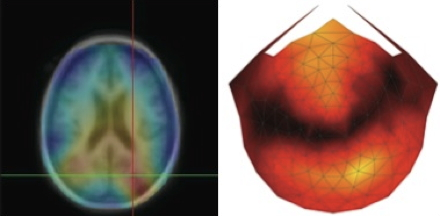
\includegraphics[width=6.11in]{img/fesi-source}

Rick O. Gilmore, Ph.D. Associate Professor of Psychology

\subsection{Today's topics}\label{todays-topics}

\begin{itemize}
\tightlist
\item
  Why neuroscience is harder than physics
\item
  Course overview
\item
  Methods in neuroscience
\end{itemize}

\section{Why neuroscience is harder than
physics}\label{why-neuroscience-is-harder-than-physics}

\begin{center}\rule{0.5\linewidth}{\linethickness}\end{center}

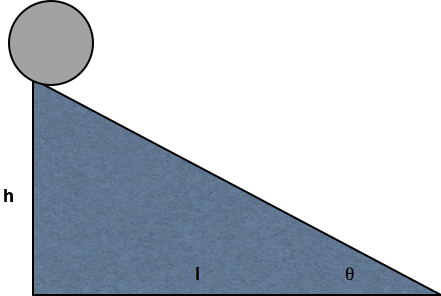
\includegraphics[width=6.12in]{img/psych-harder-1}

\begin{center}\rule{0.5\linewidth}{\linethickness}\end{center}

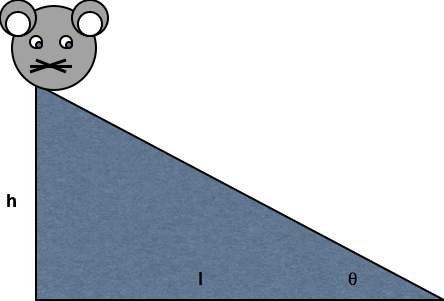
\includegraphics[width=6.17in]{img/psych-harder-2}

\subsection{What do we need to know to answer the
question?}\label{what-do-we-need-to-know-to-answer-the-question}

\begin{itemize}
\tightlist
\item
  What is the state\ldots{}

  \begin{itemize}
  \tightlist
  \item
    Of the world
  \item
    Of the organism

    \begin{itemize}
    \tightlist
    \item
      Body
    \item
      Brain/mind
    \end{itemize}
  \end{itemize}
\item
  Some states more easily measured than others
\end{itemize}

\subsection{\texorpdfstring{Brain \& behavior are complex, dynamic
\emph{systems}
with}{Brain \& behavior are complex, dynamic systems with}}\label{brain-behavior-are-complex-dynamic-systems-with}

\begin{itemize}
\tightlist
\item
  Components
\item
  Interactions
\item
  Forces/influences
\item
  Boundaries
\item
  Inputs/outputs/processes
\end{itemize}

\subsection{Systems\ldots{}}\label{systems}

\begin{itemize}
\tightlist
\item
  ``Behave'' or change state across time
\item
  Return to starting state
\item
  Appear to be regulated, controlled, influenced by feedback loops
\end{itemize}

\subsection{\texorpdfstring{May be thought of as
\href{https://en.wikipedia.org/wiki/Network_science}{networks}}{May be thought of as networks}}\label{may-be-thought-of-as-networks}


\includegraphics{https://d2ufo47lrtsv5s.cloudfront.net/content/sci/342/6158/1238411/F1.large.jpg}

\begin{center}\rule{0.5\linewidth}{\linethickness}\end{center}


\includegraphics{https://stats.idre.ucla.edu/wp-content/uploads/2016/02/sem_1.png}

\subsection{Studying systems is hard
because\ldots{}}\label{studying-systems-is-hard-because}

\begin{itemize}
\tightlist
\item
  Single parts -\textgreater{} multiple functions
\item
  Single functions -\textgreater{} multiple parts
\item
  Change structure/function over time

  \begin{itemize}
  \tightlist
  \item
    Examples?
  \end{itemize}
\item
  Biological systems not ``designed'' like human-engineered ones
\item
  Measuring what is being exchanged? What is being controlled?
\end{itemize}

\section{Course overview}\label{course-overview}

\subsection{Goals}\label{goals}

\begin{itemize}
\tightlist
\item
  Master fundamentals of neuroscientific concepts and facts
\item
  Prepare to read primary source literature in behavioral, cognitive,
  affective, and clinical neuroscience
\end{itemize}

\subsection{Structure}\label{structure}

\url{https://psu-psychology.github.io/psy-511-scan-fdns-2018}

\subsection{Questions}\label{questions}

\begin{itemize}
\tightlist
\item
  What is the basic plan of the nervous system?
\item
  How do neurons work?
\item
  How do neurons connected in networks achieve behavioral goals?
\item
  How does the nervous system develop? How has it evolved?
\end{itemize}

\subsection{Approach}\label{approach}

\subsubsection{Brain architecture
(neuroanatomy)}\label{brain-architecture-neuroanatomy}

\subsubsection{Brain function
(neurophysiology)}\label{brain-function-neurophysiology}

\subsubsection{Brain communication
(neurochemistry)}\label{brain-communication-neurochemistry}

\subsubsection{Changes over evolutionary and developmental
time}\label{changes-over-evolutionary-and-developmental-time}

\subsection{Approach}\label{approach-1}

\begin{itemize}
\tightlist
\item
  The nervous system as information processing system
\item
  \textbf{Inputs}

  \begin{itemize}
  \tightlist
  \item
    From environment, body, brain
  \end{itemize}
\item
  \textbf{Processing}

  \begin{itemize}
  \tightlist
  \item
    Current inputs + brain state + body state + possible future
    states\ldots{}
  \item
    Stored information
  \item
    Physiological \& behavioral goals
  \end{itemize}
\end{itemize}

\begin{center}\rule{0.5\linewidth}{\linethickness}\end{center}

\begin{itemize}
\tightlist
\item
  \textbf{Outputs}

  \begin{itemize}
  \tightlist
  \item
    To brain, body, environment
  \end{itemize}
\end{itemize}

\subsection{Cajal/Swanson Architecture}\label{cajalswanson-architecture}

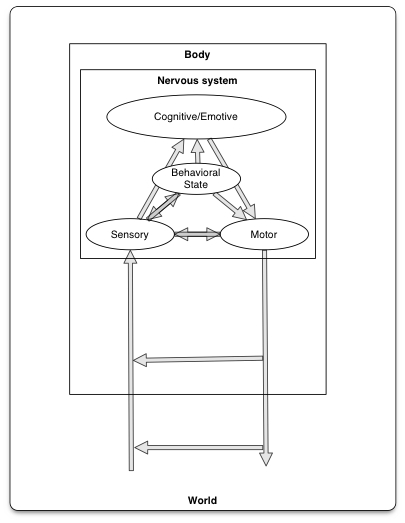
\includegraphics[width=5.62in]{img/swanson-fig-7.5}

\begin{center}\rule{0.5\linewidth}{\linethickness}\end{center}

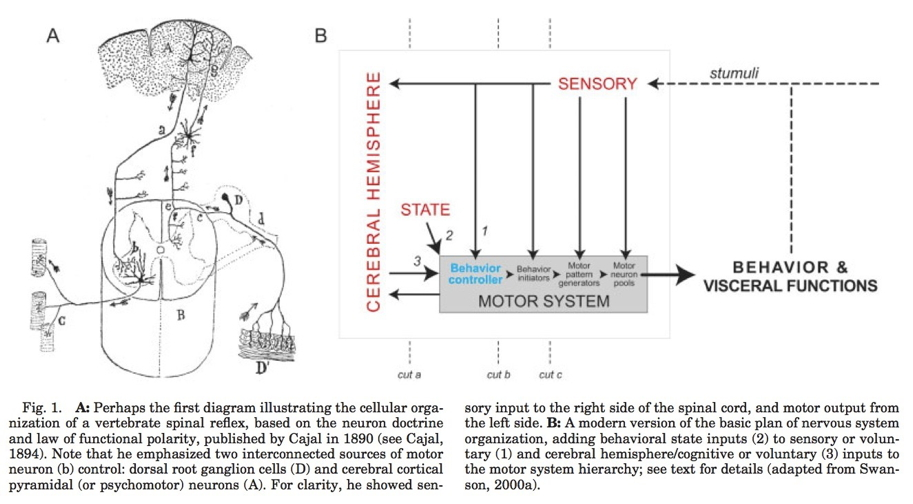
\includegraphics{https://raw.githubusercontent.com/psu-psychology/psy-511-scan-fdns-2017/master/lectures/img/swanson-2005-fig-1.jpg}

\href{http://dx.doi.org/10.1002/cne.20733}{Swanson, 2005}

\begin{center}\rule{0.5\linewidth}{\linethickness}\end{center}

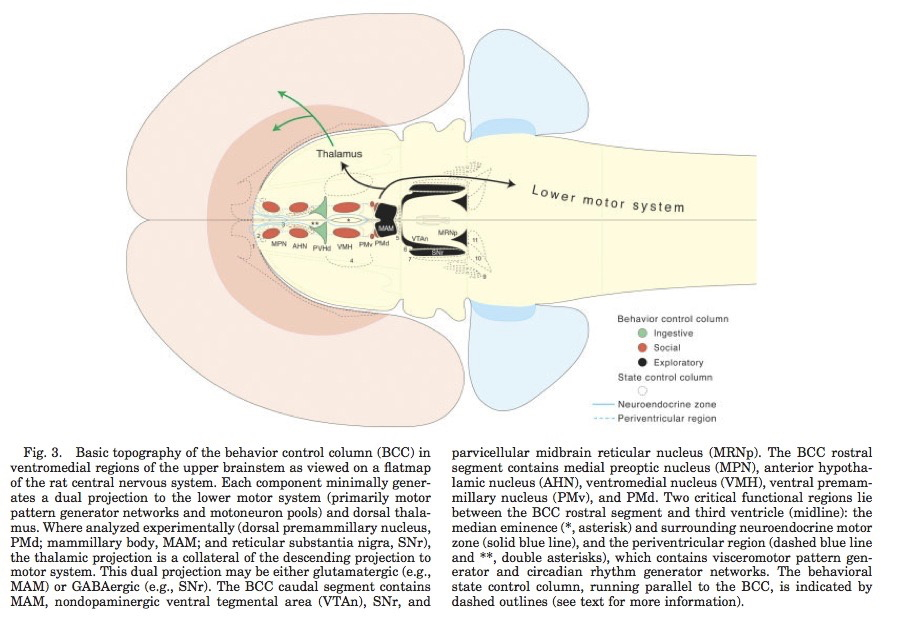
\includegraphics{https://raw.githubusercontent.com/psu-psychology/psy-511-scan-fdns-2017/master/lectures/img/swanson-2005-fig-3.jpg}

\href{http://dx.doi.org/10.1002/cne.20733}{Swanson, 2005}

\subsection{Why neuroscience needs
behavior}\label{why-neuroscience-needs-behavior}

\includegraphics{https://ars.els-cdn.com/content/image/1-s2.0-S0896627316310406-gr3.jpg}
\href{http://dx.doi.org/10.1016/j.neuron.2016.12.041}{(Krakauer et al.
2017)}

\begin{center}\rule{0.5\linewidth}{\linethickness}\end{center}

\includegraphics{https://ars.els-cdn.com/content/image/1-s2.0-S0896627316310406-gr4.jpg}

\href{http://dx.doi.org/10.1016/j.neuron.2016.12.041}{(Krakauer et al.
2017)}

\section{Neuroscience methods}\label{neuroscience-methods}

\subsection{Evaluating methods}\label{evaluating-methods}

\subsubsection{What is the question?}\label{what-is-the-question}

\begin{itemize}
\tightlist
\item
  Structure X -\textgreater{} Structure Y
\item
  Structure X -\textgreater{} Function Y
\end{itemize}

\subsubsection{What are we measuring?}\label{what-are-we-measuring}

\begin{itemize}
\tightlist
\item
  Structure
\item
  Activity

  \begin{itemize}
  \tightlist
  \item
    Why not \emph{function}?
  \end{itemize}
\end{itemize}

\subsection{Evaluating methods}\label{evaluating-methods-1}

\subsubsection{Strengths \& Weaknesses}\label{strengths-weaknesses}

\begin{itemize}
\tightlist
\item
  Cost
\item
  Invasiveness
\item
  Spatial/temporal resolution
\end{itemize}

\subsection{Spatial resolution}\label{spatial-resolution}

\includegraphics{img/churchland-levels-of-analysis.gif}

\url{http://ai.ato.ms/MITECS/Images/churchland.figure1.gif}

\subsection{\ldots{}and Temporal
Resolution}\label{and-temporal-resolution}


\includegraphics{http://www.nature.com/neuro/journal/v17/n11/images/nn.3839-F1.jpg}

\href{http://doi.org/10.1038/nn.3839}{(Sejnowski, Churchland, and
Movshon 2014)}

\subsection{Types of methods}\label{types-of-methods}

\subsubsection{Structural}\label{structural}

\begin{itemize}
\tightlist
\item
  Anatomy
\item
  Connectivity/connectome
\end{itemize}

\subsubsection{Functional (next time)}\label{functional-next-time}

\begin{itemize}
\tightlist
\item
  What does it do?
\item
  Physiology/Activity
\end{itemize}

\subsection{Mapping structures}\label{mapping-structures}

\begin{itemize}
\tightlist
\item
  Cell/axon stains
\item
  \textbf{Golgi stain} -- whole cells
\item
  Cellular distribution, concentration, microanatomy
\end{itemize}

\begin{center}\rule{0.5\linewidth}{\linethickness}\end{center}

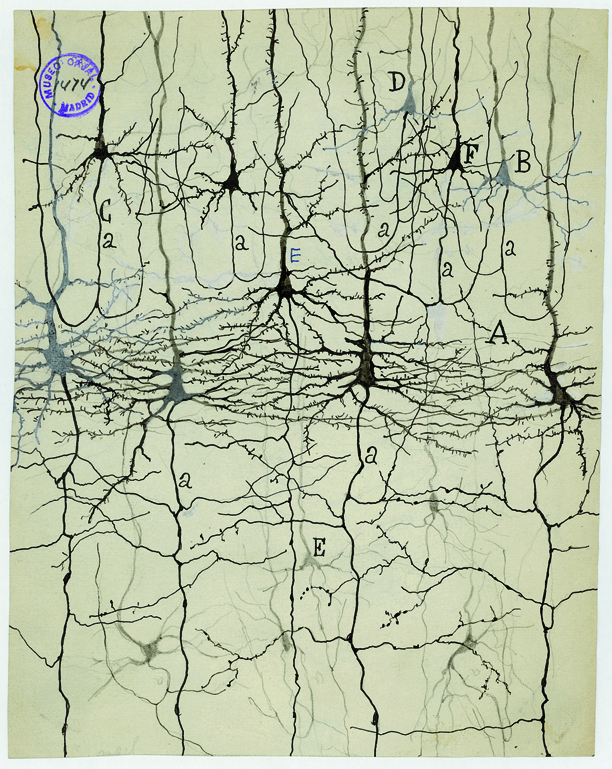
\includegraphics[width=8.5in]{img/golgi-stain}

\url{http://connectomethebook.com/wp-content/uploads/2011/11/Brainforest17_1119.jpg}

\begin{center}\rule{0.5\linewidth}{\linethickness}\end{center}

\includegraphics{https://www.hitobiotec.com/media/catalog/product/cache/1/image/9df78eab33525d08d6e5fb8d27136e95/h/i/hito_golgi_staining_10.jpg}

Here's a pretty one of the hippocampus.

\begin{center}\rule{0.5\linewidth}{\linethickness}\end{center}

\includegraphics{http://wam.umn.edu/wp-content/uploads/2016/12/WAM_Cajal_m1673.jpg}

\url{http://wam.umn.edu/calendar/cajal/}

And here is one from Santiago Ramon y Cajal.

\subsection{\texorpdfstring{\href{https://en.wikipedia.org/wiki/Camillo_Golgi}{Camillo
Golgi}}{Camillo Golgi}}\label{camillo-golgi}

\includegraphics{https://upload.wikimedia.org/wikipedia/commons/thumb/5/5f/Camillo_Golgi.jpg/330px-Camillo_Golgi.jpg}

\subsection{Nissl stain}\label{nissl-stain}

\includegraphics{https://i.pinimg.com/originals/24/ba/58/24ba5870a0b3ac2ce8e3620853e12c8b.jpg}

Here's a Nissl-stained section of the macaque brain. It stains only cell
bodies, but the density of staining tells us where there are lots of
cells and where there are fewer.

\subsection{\texorpdfstring{\href{https://en.wikipedia.org/wiki/Franz_Nissl}{Franz
Nissl}}{Franz Nissl}}\label{franz-nissl}

\subsection{Retrograde vs.~anterograde
tracers}\label{retrograde-vs.anterograde-tracers}


\includegraphics{http://openi.nlm.nih.gov/imgs/512/348/3176268/3176268_1471-2105-12-351-2.png}

\subsection{\texorpdfstring{\href{http://cbs.fas.harvard.edu/science/connectome-project/brainbow}{Brainbow}}{Brainbow}}\label{brainbow}

\href{http://doi.org/10.1038/nrn2391}{(Lichtman, Livet, and Sanes 2008)}

\subsection{Brainbow}\label{brainbow-1}

\href{http://doi.org/10.1038/nrn2391}{(Lichtman, Livet, and Sanes 2008)}

\subsection{\texorpdfstring{\href{http://clarityresourcecenter.com/CLARITY.html}{Clarity}}{Clarity}}\label{clarity}

\subsection{Evaluating cellular tracing
techniques}\label{evaluating-cellular-tracing-techniques}

\begin{itemize}
\tightlist
\item
  Invasive (in humans post-mortem only)
\item
  High spatial resolution, but poor/coarse temporal

  \begin{itemize}
  \tightlist
  \item
    Why?
  \end{itemize}
\end{itemize}

\subsection{Mapping structures}\label{mapping-structures-1}

- Computed axial tomography (CAT), CT - X-ray based

\begin{center}\rule{0.5\linewidth}{\linethickness}\end{center}

\url{http://img.tfd.com/mk/T/X2604-T-22.png}

\subsection{Tomography}\label{tomography}

\url{http://static.howstuffworks.com/gif/cat-scan-pineapple.jpg}

\begin{center}\rule{0.5\linewidth}{\linethickness}\end{center}

Here's a CT image of two brains, the one on the right has an
intracerebral hemorrhage.

\subsection{Magnetic Resonance
Imaging}\label{magnetic-resonance-imaging}

\begin{itemize}
\tightlist
\item
  Magnetic resonance a property of some isotopes and complex molecules
\item
  In magnetic field, absorb and release radio frequency energy
\item
  Hydrogen, common in water \& fat, is one
\item
  Aligns with strong magnetic field
\item
  When perturbed, speed of realignment varies by tissue
\item
  Realignment gives off radio frequency (RF) signals
\item
  Strength of RF \textasciitilde{} density
\end{itemize}

\subsection{MRI}\label{mri}

\url{http://s.hswstatic.com/gif/mri-steps.jpg}

\subsection{Structural MRI}\label{structural-mri}

\begin{itemize}
\tightlist
\item
  Tissue density/type differences
\item
  Gray vs.~white - Axon fibers
\item
  Spectroscopy
\item
  Region sizes/volumes
\end{itemize}

\begin{center}\rule{0.5\linewidth}{\linethickness}\end{center}

Here is an illustration of the different slices of an image sequence.

\begin{center}\rule{0.5\linewidth}{\linethickness}\end{center}

Here's an illustration of how different RF pulse sequences and decoding
schemes can reveal different patterns of structure.

\begin{center}\rule{0.5\linewidth}{\linethickness}\end{center}

Here's an example of MR spectroscopy showing the concentrations of
several different metabolites in a large voxel of brain tissue.

\subsection{Voxel-based morphometry
(VBM)}\label{voxel-based-morphometry-vbm}

Volume differences in schizophrenic patients vs.~controls

(Pomarol-Clotet et al. 2010)

And here's an illustration of the use of morphometric techniques. The
colored portions are statistical maps placed on top of a base structural
map. The statistical maps provide information about the comparison in
brain volumes between patients and controls in those areas.

\subsection{\texorpdfstring{What is the wiring diagram
(``connectome'')?}{What is the wiring diagram (connectome)?}}\label{what-is-the-wiring-diagram-connectome}

The idea is analogous to electronics. We want the schematic. Without the
schematic, we can't really tell what the thing does.

\begin{center}\rule{0.5\linewidth}{\linethickness}\end{center}

\subsection{Retrograde (output -\textgreater{} input) vs.~anterograde
(input -\textgreater{} output)
tracers}\label{retrograde-output---input-vs.anterograde-input---output-tracers}

\url{http://openi.nlm.nih.gov/imgs/512/348/3176268/3176268_1471-2105-12-351-2.png}

\begin{center}\rule{0.5\linewidth}{\linethickness}\end{center}

\subsection{Diffusion Tensor Imaging
(DTI)}\label{diffusion-tensor-imaging-dti}

\begin{itemize}
\tightlist
\item
  Structural MRI technique
\item
  Diffusion tensor: measurement of spatial pattern of \(H_2O\) diffusion
  in small volume
\item
  Uniform (``isotropic'') vs.~non-uniform (``anisotropic'')
\item
  Strong anisotropy suggests large \# of axons with similar orientations
  (fiber tracts)
\end{itemize}

\begin{center}\rule{0.5\linewidth}{\linethickness}\end{center}

Here's an illustration of what a tensor looks like. You can see an
isotropic and an anisotropic tensor.

\begin{center}\rule{0.5\linewidth}{\linethickness}\end{center}

And here's how we go from a tensor to estimating the pathway of a fiber
tract.

\begin{center}\rule{0.5\linewidth}{\linethickness}\end{center}

\subsection{Connectome as matrix}\label{connectome-as-matrix}

\begin{center}\rule{0.5\linewidth}{\linethickness}\end{center}

\subsection{Main points}\label{main-points}

\begin{itemize}
\tightlist
\item
  Psychology is harder than physics
\item
  Understanding brain/behavior relations requires a diverse toolkit
\end{itemize}

\subsection{Your turn}\label{your-turn}

\begin{enumerate}
\def\labelenumi{\arabic{enumi}.}
\tightlist
\item
  Pick two papers you want to read and (better) understand

  \begin{itemize}
  \tightlist
  \item
    Email me APA formatted citation (with DOIs)
  \item
    Indicate three concepts/terms you are especially interested in
    understanding
  \end{itemize}
\item
  Choose a behavior or mental state you want to (better) understand

  \begin{itemize}
  \tightlist
  \item
    Take an information processing perspective and briefly sketch out
    (in no more than a short paragraph) the main inputs, outputs, and
    computations involved.
  \item
    When thinking about \emph{outputs} make sure to distinguish between
    \emph{behaviors} (e.g., movements, facial expressions,
    vocalizations) and \emph{physiological states} (e.g., changes in
    heart rate, hormone concentrations in the blood, etc.)
  \end{itemize}
\end{enumerate}

\subsection*{References}\label{references}
\addcontentsline{toc}{subsection}{References}

\hypertarget{refs}{}
\hypertarget{ref-Krakauer2017-xl}{}
Krakauer, John W, Asif A Ghazanfar, Alex Gomez-Marin, Malcolm A MacIver,
and David Poeppel. 2017. ``Neuroscience Needs Behavior: Correcting a
Reductionist Bias.'' \emph{Neuron} 93 (3): 480--90.
doi:\href{https://doi.org/10.1016/j.neuron.2016.12.041}{10.1016/j.neuron.2016.12.041}.

\hypertarget{ref-lichtman_technicolour_2008}{}
Lichtman, Jeff W., Jean Livet, and Joshua R. Sanes. 2008. ``A
Technicolour Approach to the Connectome.'' \emph{Nature Reviews
Neuroscience} 9 (6): 417--22.
doi:\href{https://doi.org/10.1038/nrn2391}{10.1038/nrn2391}.

\hypertarget{ref-Pomarol-Clotet2010-tq}{}
Pomarol-Clotet, E, E J Canales-Rodríguez, R Salvador, S Sarró, J J
Gomar, F Vila, J Ortiz-Gil, Y Iturria-Medina, A Capdevila, and P J
McKenna. 2010. ``Medial Prefrontal Cortex Pathology in Schizophrenia as
Revealed by Convergent Findings from Multimodal Imaging.'' \emph{Mol.
Psychiatry} 15 (8): 823--30.
doi:\href{https://doi.org/10.1038/mp.2009.146}{10.1038/mp.2009.146}.

\hypertarget{ref-sejnowski2014putting}{}
Sejnowski, Terrence J, Patricia S Churchland, and J Anthony Movshon.
2014. ``Putting Big Data to Good Use in Neuroscience.'' \emph{Nature
Neuroscience} 17 (11). Nature Publishing Group: 1440--1.
doi:\href{https://doi.org/10.1038/nn.3839}{10.1038/nn.3839}.


\end{document}
